\documentclass{vldb}
\usepackage{graphicx}
\usepackage{url}
\usepackage{caption}
\usepackage{float}


\begin{document}

% ****************** TITLE ****************************************

\title{Assignment 4 - DB2}

% ****************** AUTHORS **************************************

\numberofauthors{2} 

\author{
% 1st. author
\alignauthor Daniel Brand
% 2nd. author
\alignauthor Andreas Kostecka
}

\maketitle

\section{Recovery-Methods}
Whenever an application error, power interruption or storage failure happens the database has to be rebuilt. For this case it is very important to backup the whole database or individual table spaces to rebuild damaged, broken or corrupted data. \\\\
There are three types of recovery:
\begin{itemize}
\item Crash-Recovery
\begin{itemize}
\item When transactions (also called UOW, units of work) are interrupted unexpected the database may have an inconsistent or unusable state. Crash-Recovery deals with such problems. 
\end{itemize}
\item Version-Recovery
\begin{itemize}
\item Version-Recovery describes the restoration of a previous version of the database. For this recovery type DB2 needs an image that was created during a backup operation.
\end{itemize}
\item Rollforward-Recovery
\begin{itemize}
\item Rollforward-Recovery can be used to reapply changes that were made by transactions that were committed after a backup was made.
\end{itemize}
\end{itemize}

After a power interruption the DB2 Database-Manager starts automatically the Crash-Recovery routine.\footnote{\url{https://www-01.ibm.com/support/knowledgecenter/?lang=de#!/SSEPGG_9.7.0/com.ibm.db2.luw.admin.ha.doc/doc/c0052073.html}}

\section{Backup and Recovery-Strategy}
For an backup and recovery strategy we should ask ourselves some questions:\\
Will the database be recoverable?
How much time can be spent recovering the database?
How much time will pass between backup operations?
How much storage space can be allocated for backup copies and archived logs?
Will table space level backups be sufficient, or will full database backups be necessary? and so on.\footnote{\url{https://www-01.ibm.com/support/knowledgecenter/?lang=de#!/SSEPGG_9.7.0/com.ibm.db2.luw.admin.ha.doc/doc/c0005945.html}}\\
A strategy for recovering a database should ensure that all the informations needed for the recovery process are available to the system. A strategy should also contain a timetable for periodically backups.

\subsection{Recovery-Methods in Detail}
\begin{itemize}
\item Database-Backup:\footnote{\url{http://myy.haaga-helia.fi/~dbms/db2/01_Classroom/2.1\%20-\%20DB2\%20backup\%20and\%20recovery_Lab.pdf}}\\
Copying and saving the copy of the data on a different drive. If the original data gets corrupted we can easily restore the database. A simple way to generate a backup is to stop the database to ensure that there are no more active transactions and then creating a backup-image from the original data. 
\item Database-Recovery:\\
The recreation of the database is called recovery. Version recovery is the restoration of a previous version of the database. Rollforward recovery is the re-running of all protocoled transactions after the recovery of a database or table space. 
\item Recovery after system crash:\\
A recovery after a system crash is a so called automatic recovery of the database. Transactions against a database can be interrupted unexpectedly when a system crash happens. When this crash occurs before all of the changes made by the transactions are finished and committed, the database has an inconsistent and unusable state. The automatic crash recovery routine established first a connection to the database. After that the database logs are used to restore the database to a consistent state. Database changes performed by transactions that are incomplete gets rolled back and also completing committed transactions that are still in memory when the crash occurred (Figure \ref{fig:crecovery}). Also data page externalization is performed for all committed transactions. At the end of the crash recovery the DB2 database is restored into a transaction consistent state. If necessary damaged table spaces are also fixed. 
\begin{figure}[H]
	\centering
	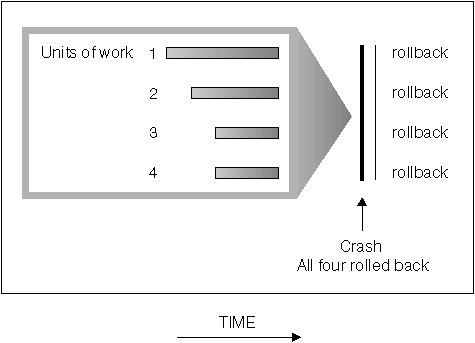
\includegraphics[width=.38\textwidth]{crash-recover.png}
	\caption{Crash-Recovery}
	\label{fig:crecovery}
\end{figure}
\item Log-Files (seen in Figure \ref{fig:dbfiles}):
\begin{itemize}
\item Recovery log files: The DB2 \textbf{Recovery log files} tracks all of the changes made against the database. It is also called the transaction log. A transaction is invoked whenever one of the following operations is executed: insert, read, update, delete data. First the record is copied to the buffer pool, where it is modified by the chosen operation. Once a record is modified due to one of these operation a new record reflecting the operation is written to the log buffer. The log buffer is a storage are in the memory. On a delete operation the record containing the original values is written to the log buffer. 
\item Recovery history files: The DB2 \textbf{Recovery history file} is created for each database and updated during various operations. These operations could be: table spaces are backed up, restored or rolled forward; table space is created, altered, renamed, dropped; table is loaded, dropped or reorganized; database is recovered; log file is created or archived.
\item Table space history files: The \textbf{Table space history files} keeps track of which logs need to be included and processed for each table space. For example DB2 uses the table space history and log files for recovering a dropped table (is done via table space level restore). When we create a backup also the history files are backed up. Each entry in the history file has an associated status: active, inactive, expired, pending, delete, deleted, and do\_not\_delete.
\end{itemize}
\end{itemize}

\begin{figure}[H]
	\centering
	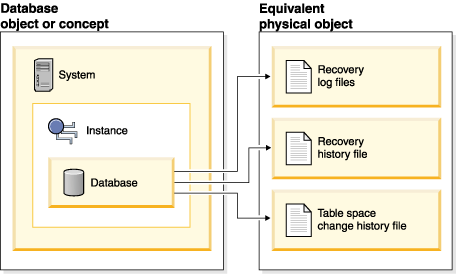
\includegraphics[width=.38\textwidth]{db-files.png}
	\caption{Database-Logs}
	\label{fig:dbfiles}
\end{figure}

\subsection{Automated Backup Operations}
It is very time consuming to determine whenever a backup-operation should be executed. DB2 offers a Configure Automatic Maintenance wizard for doing automatically backups. With automatic maintenance, you specify your maintenance objectives, including when automatic maintenance can run. It is still possible to perform a manual backup. 

\subsection{Monitoring}
To monitor the progress of backup, restore and recovery operations DB2 offers the following command\footnote{\url{https://www-01.ibm.com/support/knowledgecenter/?lang=en#!/SSEPGG_9.7.0/com.ibm.db2.luw.admin.ha.doc/doc/t0011701.html}}:
\begin{verbatim}
LIST UTILITIES SHOW DETAIL
\end{verbatim}

This command displays the progress information of all active utilities on the corresponding instance. The information contains the type of the activity (backup, recover, restore, rollforward), database name, description for the type (eg. offline backup), start time, state (eg. executing, finished ...),who invokes the operation (eg. user, system ...), priority. Also some information about the progress monitoring: percentage complete, total work, already completed work.    

\section{Backup}
For a simple backup operation we only need the alias of the database and the following command:
\begin{verbatim}
db2 backup db alias_name_db
\end{verbatim}

If not specified the backup is stored in the directory where the command is executed. It is possible to save backups in:
\begin{itemize}
\item A directory (for backups to disk or diskette)
\item A device (for backups to tape)
\item A Tivoli Storage Manager (TSM) server
\item Another vendor's server
\end{itemize}

The recovery history file is updated automatically with summary information whenever you invoke a database backup operation. This file is created in the same directory as the database configuration file.\\

With the tool \textbf{db2ckbkp} we can display information about existing backup images. This tool can test the integrity of backups, display the backup-header and display information about the objects and the log file header in the backup image.

\section{Recover vs Restore and Rollforward}
With \textbf{RESTORE}, you specify the backup image you want to restore (indicated by the timestamp the backup was TAKEN AT) the media you are restoring from and the database name you are restoring to. Then if you want to roll the database forward to end of logs or a point in time you follow the restore with a \textbf{ROLLFORWARD} command.\\\\ The \textbf{RECOVER} command combines the two statements above and makes it also simpler to specify a certain backup-goal.\\

For example if you simply want to get the database back to the end of the log files that exist you simply run:

 \begin{verbatim}
db2 RECOVER DATABASE db_name TO END OF LOGS
\end{verbatim}

DB2 searches automatically for the last corresponding backup and invokes the \textbf{RESTORE} command with all the needed parameter. After the \textbf{RESTORE} is executed the \textbf{RECOVER} command invokes \textbf{ROLLFORWARD} to the end of logs. 

\end{document}

